			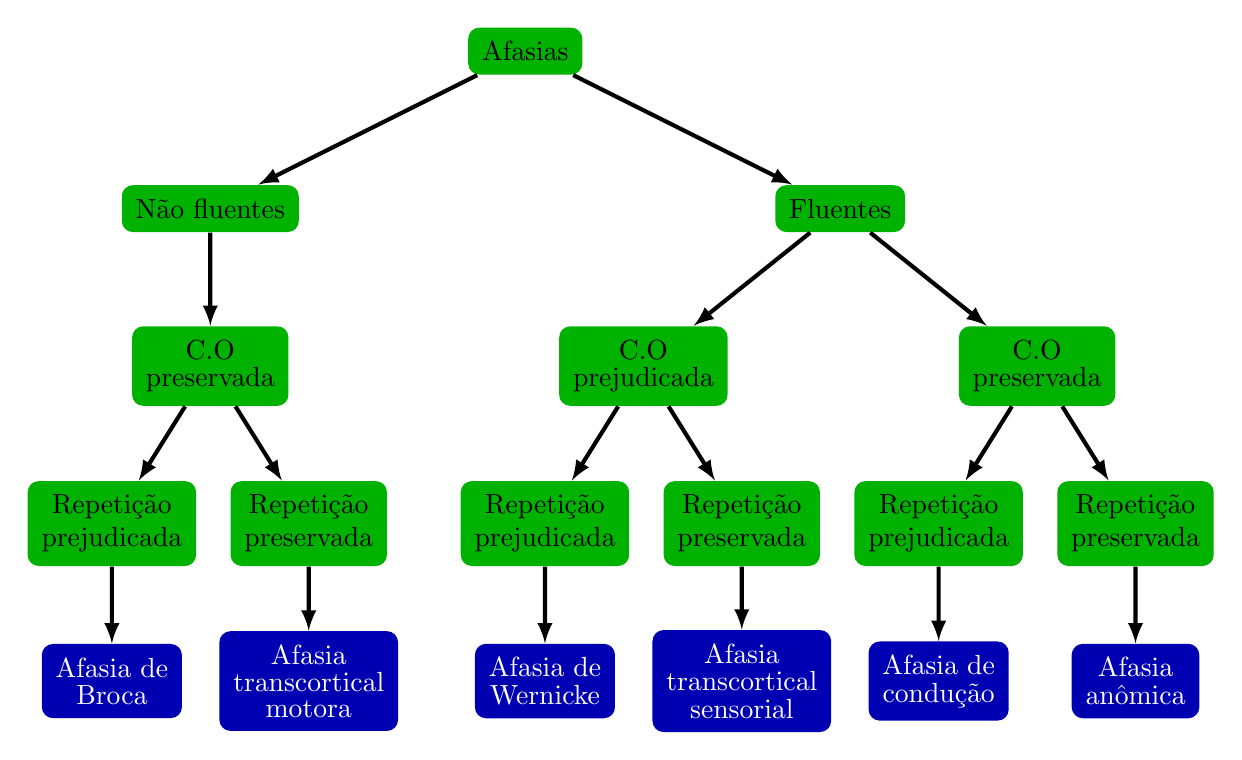
\begin{tikzpicture}[
	level 1/.style={level distance=20mm, sibling distance=80mm},
	level 2/.style={level distance=20mm, sibling distance=50mm},
	level 3/.style={level distance=20mm, sibling distance=25mm},
	edge from parent/.style={
		->,
		draw,
		line width=1.5pt % Adjust the line width here
	},
	>=latex,
	every node/.style={
		rectangle, 
		draw=none, 
		align=center, 
		rounded corners,
		inner sep=5pt,
		fill=green!70!black, text=black
	},
	% Style for the last level
	last_level_style/.style={
		fill=blue!70!black, % Change color here
		text=white
	}
	]
	\node {Afasias}
	child {
		node {Não fluentes}
		child {
			node {\shortstack{C.O\\preservada}}
			child {
				node {\shortstack{Repetição\\prejudicada}}
				child {
					node[last_level_style] {\shortstack{Afasia de\\Broca}}
				}
			}
			child {
				node {\shortstack{Repetição\\preservada}}
				child {
					node[last_level_style] {\shortstack{Afasia \\transcortical \\motora}}
				}
			}
		}
	}
	child {
		node {Fluentes}
		child {
			node {\shortstack{C.O\\prejudicada}}
			child {
				node {\shortstack{Repetição\\prejudicada}}
				child {
					node[last_level_style] {\shortstack{Afasia de \\Wernicke}}
				}
			}
			child {
				node {\shortstack{Repetição\\preservada}}
				child {
					node[last_level_style] {\shortstack{Afasia \\transcortical \\sensorial}}
				}
			}
		}
		child {
			node {\shortstack{C.O\\preservada}}
			child {
				node {\shortstack{Repetição\\prejudicada}}
				child {
					node[last_level_style] {\shortstack{Afasia de \\condução}}
				}
			}
			child {
				node {\shortstack{Repetição\\preservada}}
				child {
					node[last_level_style] {\shortstack{Afasia \\anômica}}
				}
			}
		}
	};
\end{tikzpicture}